\documentclass[letterpaper,12pt,fleqn]{article}
\usepackage{matharticle}
\usepackage{mathtools}
\usepackage{polynom}
\usepackage{tikz}
\pagestyle{plain}
\begin{document}

\begin{center}
\Large Math-19 Homework \#5 Solutions
\end{center}

\vspace{0.5in}

\underline{Reading}

Please read sections 3.1 through 3.7, omitting 3.5, and do all concept problems
in the posted sections on web\-assign.

\underline{Problems}

\begin{enumerate}
\item Let $f(x)=1-6x-x^2$.
\begin{enumerate}
\item Convert the parabola to standard form.
\begin{eqnarray*}
f(x) &=& 1-6x-x^2 \\
    &=& -(x^2+6x)+1 \\
    &=& -(x^2+6x+9)+1+9 \\
    &=& -(x+3)^2+10 \\
\end{eqnarray*}

\item What are the coordinates of the vertex?
\[(-3,10)\]

\item What are the x-intercepts (if any)?
\begin{eqnarray*}
-(x+3)^2+10 &=& 0 \\
(x+3)^2 &=& 10 \\
x+3 &=& \pm\sqrt{10} \\
x &=& -3\pm\sqrt{10} \\
\end{eqnarray*}
\[(-3\pm\sqrt{10},0)\]

\item What are the y-intercepts (if any)?
\[f(0)=1-6(0)-0^2=1\]
\[(0,1)\]

\item What is the axis of symmetry?
\[x=-3\]
\newpage
\item Sketch the parabola. Be sure to label the vertex and all intercepts!

\begin{tikzpicture}[scale=0.5]
\draw [<->] (-10,0) -- (10,0);
\draw [<->] (0,-10) -- (0,10,0);
\draw [dashed] (-3,10) -- (-3,-10);
\draw [fill=black] (-3,10) circle [radius=0.1];
\draw [fill=black] (0,1) circle [radius=0.1];
\draw [fill=black] (-6.16228,0) circle [radius=0.1];
\draw [fill=black] (0.16228,0) circle [radius=0.1];
\draw [domain=-7.5:1.5] plot ({\x},{1-6*(\x)-(\x)^2});
\node [above] at (-3,10) {$(-3,10)$};
\node [left] at (0,1) {$(0,1)$};
\node [below right] at (0.16228,0) {$(-3+\sqrt{10},0)$};
\node [below left] at (-6.16228,0) {$(-3-\sqrt{10},0)$};
\node [below] at (-3,-10) {$x=-3$};
\end{tikzpicture}

\item What is the domain?
\[\R\]

\item What is the range?
\[(-\infty,10]\]
\end{enumerate}

\item Let $p(x)=10-49x+80x^2-53x^3+20x^4-4x^5$. Factor completely. Use the
results of the factoring and any y-intercepts to sketch the function. Be sure
to label all intercepts!
\[p=\pm1,\pm2,\pm5,\pm10\]
\[q=\pm1,\pm2,\pm4\]

\[p(1)=4\ne0\]
\[p(-1)=216\ne0\]
\[p(2)=0\]

\polylongdiv{-4x^5+20x^4-53x^3+80x^2-49x+10}{x-2}

\[p(x)=(x-2)q(x)=(x-2)(-4x^4+12x^3-29x^2+22x-5)\]

\[p=\pm1,\pm5\]
\[q=\pm1,\pm2,\pm4\]

We already know $\pm1$ doesn't work.

\[q(5)=-1620\ne0\]
\[q(-5)=-4840\ne0\]
\[q\left(\frac{1}{2}\right)=0\]

The factor is $\left(x-\frac{1}{2}\right)$; however, we can factor out the
$\frac{1}{2}$ and use $(2x-1)$.

\polylongdiv{-4x^4+12x^3-29x^2+22x-5}{2x-1}

\[p(x)=(x-2)(2x-1)r(x)=(x-2)(2x-1)(-2x^3+5x^2-12x+5)\]

\[p=\pm1,\pm5\]
\[q=\pm1,\pm2\]

We already know that $\pm1$ and $\pm5$ don't work, but we need to retry
$\frac{1}{2}$, just in case it is a repeated root.

\[r\left(\frac{1}{2}\right)=0\]

\polylongdiv{-2x^3+5x^2-12x+5}{2x-1}

\[p(x)=(x-2)(2x-1)^2(-x^2+2x-5)=-(x-2)(2x-1)^2(x^2-2x+5)\]

Notice that the leading coefficient will be correct:
\[-x\cdot(2x)^2\cdot x^2=-4x^5\]

Also note that the final quadratic does not factor in the reals. So, we use
our calculator and find that this quadratic doesn't introduce any more humps
(see graph for next problem).

So, we have x-intercepts at $(1/2,0)$ and $(2,0)$ and a y-intercept at (0,10).

\begin{tikzpicture}[scale=0.5]
\draw [<->] (-5,0) -- (5,0);
\draw [<->] (0,-5) -- (0,15);
\draw [fill=black] (0.5,0) circle [radius=0.1];
\draw [fill=black] (2,0) circle [radius=0.1];
\draw [fill=black] (0,10) circle [radius=0.1];
\draw [domain=-0.1:2.1]
    plot ({\x},{10-49*(\x)+80*(\x)^2-53*(\x)^3+20*(\x)^4-4*(\x)^5});
\node [above right] at (0,10) {$10$};
\node [below] at (0.5,0) {$\frac{1}{2}$};
\node [below right] at (2,0) {$2$};
\end{tikzpicture}

\item For the previous problem, graph the function using your calculator. You
will need to play with the window a bit so that you can see the important
detail. Determine all local maxima/minima and attach screenshots.

We already know that we have a local minimum at $(1/2,0)$. For the remaining
local maximum, see the graph.

\item Let:
\[f(x)=\frac{(2x^2+2x-4)(x+3)}{x^4+4x^3+3x^2}\]
\begin{enumerate}
\item What are the zeros?

\begin{eqnarray*}
f(x) &=& \frac{(2x^2+2x-4)(x+3)}{x^4+4x^3+3x^2} \\
     &=& \frac{2(x^2+x-2)(x+3)}{x^2(x^2+4x+3)} \\
     &=& \frac{2(x+2)(x-1)(x+3)}{x^2(x+1)(x+3)} \\
     &=& \frac{2(x+2)(x-1)}{x^2(x+1)}\hspace{0.5in}x\ne-3 \\
\end{eqnarray*}
\[(-2,0), (1,0)\]

\item What are the vertical asymptotes (if any)?
\[x=-1, x=0\]

\item What are the horizontal asymptotes (if any)?

\bigskip

The numerator is degree=2 and the denominator is degree=3.

$2<3$

So, there is a horizontal asymptote at $y=0$ (the x-axis).

\bigskip

\item What is the end behavior as $x\to\infty$?
\[f(x)\to\frac{2\cdot+\cdot+}{+\cdot+}\to+\]
\[f(x)\to0^+\]

\item What is the end behavior as $x\to-\infty$?
\[f(x)\to\frac{2\cdot-\cdot-}{+\cdot-}\to-\]
\[f(x)\to0^-\]

\item What are the y-intercepts (if any)?

\bigskip

none ($x=0$ is a vertical asymptote).

\bigskip

\item Sketch the graph. Be sure to label all intercepts, asymptotes, and
local extrema and show the proper end behavior. Note that you may need to use a
calculator to determine the local extrema.

\begin{tikzpicture}[scale=0.5]
\draw [<->] (-10,0) -- (10,0);
\draw [<->] (0,-10) -- (0,10);
\draw [dashed] (-1,-10) -- (-1,10);
\draw [fill=black] (-2,0) circle [radius=0.1];
\draw [fill=black] (1,0) circle [radius=0.1];
\draw [fill=black] (-0.678363,-2.9735) circle [radius=0.1];
\draw [fill=black] (-3.17241,-0.447485) circle [radius=0.1];
\draw [fill=black] (1.85577,0.671006) circle [radius=0.1];
\draw [domain=-10:-1.25] plot ({\x},{(2*((\x)+2)*((\x)-1))/((\x)^2*((\x)+1))});
\draw [domain=0.45:10] plot ({\x},{(2*((\x)+2)*((\x)-1))/((\x)^2*((\x)+1))});
\draw [domain=-0.83:-0.49]
    plot ({\x},{(2*((\x)+2)*((\x)-1))/((\x)^2*((\x)+1))+27});
\node [above left] at (-2,0) {$(-2,0)$};
\node [below right] at (1,0) {$(1,0)$};
\node [above left] at (-1,10) {$x=-1$};
\node [above right] at (0,10) {$x=0$};
\node [right] at (10,0) {$y=0$};
\node [right] at (-0.678363,-2.9735) {$(-0.68,-29.97)$};
\node [above right] at (1.85577,0.671006) {$(1.86,0.67)$};
\draw [fill=white] (-3,-0.44444) circle [radius=0.1];
\node [below right] at (-3,-0.44444) {$(-3,-0.444)$};
\node [below left] at (-3.17241,-0.444785) {$(-3.17,-0.447)$};
\end{tikzpicture}

\item What is the domain?
\[(-\infty,-3)\cup(-3,-1)\cup(-1,0)\cup(0,\infty)\]

\item What is the range?
\[\R\]
\end{enumerate}

\item Solve for $x$:
\[\frac{x+2}{x+3}<\frac{x-1}{x-2}\]
Remember to state the result in interval notation.

\begin{eqnarray*}
\frac{x+2}{x+3}-\frac{x-1}{x-2} &<& 0 \\
\frac{x+2}{x+3}-\frac{x-1}{x-2} &<& 0 \\
\frac{(x+2)(x-2)-(x+3)(x-1)}{(x+3)(x-2)} &<& 0 \\
\frac{(x^2-4)-(x^2+2x-3)}{(x+3)(x-2)} &<& 0 \\
\frac{-2x-1}{(x+3)(x-2)} &<& 0 \\
\frac{2x+1}{(x+3)(x-2)} &>& 0 \\
\end{eqnarray*}

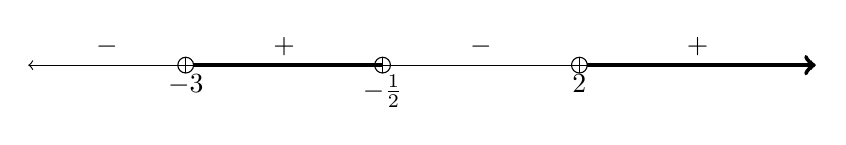
\begin{tikzpicture}
\draw [<->] (-5,0) -- (5,0);
\draw (-0.5,-0.1) -- (-0.5,0.1);
\draw (-3,-0.1) -- (-3,0.1);
\draw (2,-0.1) -- (2,0.1);
\draw (-0.5,0) circle [radius=0.1];
\draw (-3,0) circle [radius=0.1];
\draw (2,0) circle [radius=0.1];
\node [below] at (-0.5,0) {$-\frac{1}{2}$};
\node [below] at (-3,0) {$-3$};
\node [below] at (2,0) {$2$};
\node [above] at (-4,0) {$-$};
\node [above] at (-1.75,0) {$+$};
\node [above] at (0.75,0) {$-$};
\node [above] at (3.5,0) {$+$};
\draw [ultra thick] (-2.9,0) -- (-0.5,0);
\draw [ultra thick,->] (2.1,0) -- (5,0);
\end{tikzpicture}

\[(-3,-\frac{1}{2})\cup(2,\infty)\]
\end{enumerate}
\end{document}
